14. \begin{figure}[ht!]
\center{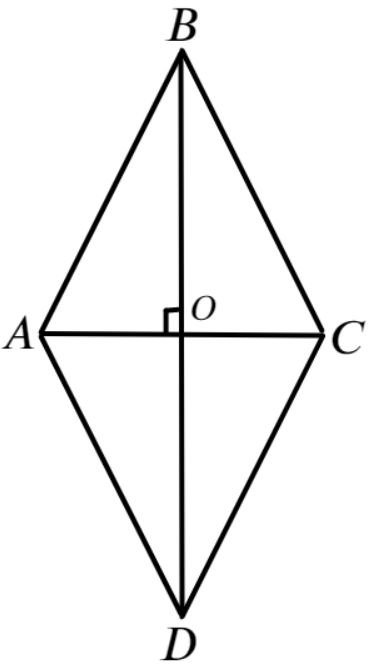
\includegraphics[scale=0.35]{g8-13.png}}
\end{figure}\\
Диагонали ромба перпендикулярны и делятся точкой пересечения пополам. Пусть $BO=\cfrac{1}{2}\cdot4\sqrt{3}=2\sqrt{3}$ и $AO=\cfrac{1}{2}\cdot4=2.$ Тогда $tg(\angle ABO)=\cfrac{2}{2\sqrt{3}}=\cfrac{\sqrt{3}}{3}\Rightarrow \angle ABO =30^\circ,\ \angle B=60^\circ,\ \angle D=\angle B=60^\circ,\ \angle A=\angle C=180^\circ-60^\circ=120^\circ.$\\
